\documentclass[11pt]{mimosis}
% \PassOptionsToClass{14pt}{scrbook}
\usepackage{metalogo}

\usepackage{textcomp}
\usepackage{gensymb}

%%%%%%%%%%%%%%%%%%%%%%%%%%%%%%%%%%%%%%%%%%%%%%%%%%%%%%%%%%%%%%%%%%%%%%%%
% Some of my favorite personal adjustments
%%%%%%%%%%%%%%%%%%%%%%%%%%%%%%%%%%%%%%%%%%%%%%%%%%%%%%%%%%%%%%%%%%%%%%%%
%
% These are the adjustments that I consider necessary for typesetting
% a nice thesis. However, they are *not* included in the template, as
% I do not want to force you to use them.

% This ensures that I am able to typeset bold font in table while still aligning the numbers
% correctly.
\usepackage{etoolbox}

\usepackage[binary-units=true]{siunitx}
\DeclareSIUnit\px{px}

\sisetup{%
  detect-all           = true,
  detect-family        = true,
  detect-mode          = true,
  detect-shape         = true,
  detect-weight        = true,
  detect-inline-weight = math,
}

%%%%%%%%%%%%%%%%%%%%%%%%%%%%%%%%%%%%%%%%%%%%%%%%%%%%%%%%%%%%%%%%%%%%%%%%
% Hyperlinks & bookmarks
%%%%%%%%%%%%%%%%%%%%%%%%%%%%%%%%%%%%%%%%%%%%%%%%%%%%%%%%%%%%%%%%%%%%%%%%

\usepackage[%
  colorlinks = true,
  citecolor  = Black,
  linkcolor  = Black,
  urlcolor   = Black,
  ]{hyperref}

\usepackage{bookmark}


%%%%%%%%%%%%%%%%%%%%%%%%%%%%%%%%%%%%%%%%%%%%%%%%%%%%%%%%%%%%%%%%%%%%%%%%
% Bibliography
%%%%%%%%%%%%%%%%%%%%%%%%%%%%%%%%%%%%%%%%%%%%%%%%%%%%%%%%%%%%%%%%%%%%%%%%
%
% I like the bibliography to be extremely plain, showing only a numeric
% identifier and citing everything in simple brackets. The first names,
% if present, will be initialized. DOIs and URLs will be preserved.

\usepackage[%
  autocite     = plain,
  backend      = bibtex,
  doi          = true,
  url          = true,
  giveninits   = true,
  hyperref     = true,
  maxbibnames  = 99,
  maxcitenames = 99,
  sortcites    = true,
  style        = alphabetic,
  citestyle    = alphabetic,
  backref      = true,
  ]{biblatex}


%%%%%%%%%%%%%%%%%%%%%%%%%%%%%%%%%%%%%%%%%%%%%%%%%%%%%%%%%%%%%%%%%%%%%%%%
% Some adjustments to make the bibliography more clean
%%%%%%%%%%%%%%%%%%%%%%%%%%%%%%%%%%%%%%%%%%%%%%%%%%%%%%%%%%%%%%%%%%%%%%%%
%
% The subsequent commands do the following:
%  - Removing the month field from the bibliography
%  - Fixing the Oxford commma
%  - Suppress the "in" for journal articles
%  - Remove the parentheses of the year in an article
%  - Delimit volume and issue of an article by a colon ":" instead of
%    a dot ""
%  - Use commas to separate the location of publishers from their name
%  - Remove the abbreviation for technical reports
%  - Display the label of bibliographic entries without brackets in the
%    bibliography
%  - Ensure that DOIs are followed by a non-breakable space
%  - Use hair spaces between initials of authors
%  - Make the font size of citations smaller
%  - Fixing ordinal numbers (1st, 2nd, 3rd, and so) on by using
%    superscripts

% Remove the month field from the bibliography. It does not serve a good
% purpose, I guess. And often, it cannot be used because the journals
% have some crazy issue policies.
\AtEveryBibitem{\clearfield{month}}
\AtEveryCitekey{\clearfield{month}}

% Fixing the Oxford comma. Not sure whether this is the proper solution.
% More information is available under [1] and [2].
%
% [1] http://tex.stackexchange.com/questions/97712/biblatex-apa-style-is-missing-a-comma-in-the-references-why
% [2] http://tex.stackexchange.com/questions/44048/use-et-al-in-biblatex-custom-style
%
\AtBeginBibliography{%
  \renewcommand*{\finalnamedelim}{%
    \ifthenelse{\value{listcount} > 2}{%
      \addcomma
      \addspace
      \bibstring{and}%
    }{%
      \addspace
      \bibstring{and}%
    }
  }
}

% Suppress "in" for journal articles. This is unnecessary in my opinion
% because the journal title is typeset in italics anyway.
\renewbibmacro{in:}{%
  \ifentrytype{article}
  {%
  }%
  % else
  {%
    \printtext{\bibstring{in}\intitlepunct}%
  }%
}

% Remove the parentheses for the year in an article. This removes a lot
% of undesired parentheses in the bibliography, thereby improving the
% readability. Moreover, it makes the look of the bibliography more
% consistent.
\renewbibmacro*{issue+date}{%
  \setunit{\addcomma\space}
    \iffieldundef{issue}
      {\usebibmacro{date}}
      {\printfield{issue}%
       \setunit*{\addspace}%
       \usebibmacro{date}}%
  \newunit}

% Delimit the volume and the number of an article by a colon instead of
% by a dot, which I consider to be more readable.
\renewbibmacro*{volume+number+eid}{%
  \printfield{volume}%
  \setunit*{\addcolon}%
  \printfield{number}%
  \setunit{\addcomma\space}%
  \printfield{eid}%
}

% Do not use a colon for the publisher location. Instead, connect
% publisher, location, and date via commas.
\renewbibmacro*{publisher+location+date}{%
  \printlist{publisher}%
  \setunit*{\addcomma\space}%
  \printlist{location}%
  \setunit*{\addcomma\space}%
  \usebibmacro{date}%
  \newunit%
}

% Ditto for other entry types.
\renewbibmacro*{organization+location+date}{%
  \printlist{location}%
  \setunit*{\addcomma\space}%
  \printlist{organization}%
  \setunit*{\addcomma\space}%
  \usebibmacro{date}%
  \newunit%
}

% Do not abbreviate "technical report".
\DefineBibliographyStrings{english}{%
  techreport = {technical report},
}

% Display the label of a bibliographic entry in bare style, without any
% brackets. I like this more than the default.
%
% Note that this is *really* the proper and official way of doing this.
\DeclareFieldFormat{labelnumberwidth}{#1\adddot}

% Ensure that DOIs are followed by a non-breakable space.
\DeclareFieldFormat{doi}{%
  \mkbibacro{DOI}\addcolon\addnbspace
    \ifhyperref
      {\href{http://dx.doi.org/#1}{\nolinkurl{#1}}}
      %
      {\nolinkurl{#1}}
}

% Use proper hair spaces between initials as suggested by Bringhurst and
% others.
\renewcommand*\bibinitdelim {\addnbthinspace}
\renewcommand*\bibnamedelima{\addnbthinspace}
\renewcommand*\bibnamedelimb{\addnbthinspace}
\renewcommand*\bibnamedelimi{\addnbthinspace}

% Make the font size of citations smaller. Depending on your selected
% font, you might not need this.
\renewcommand*{\citesetup}{%
  \biburlsetup
  \small
}

% \DeclareLanguageMapping{british}{bibliography-correct-ordinals}
% \DeclareLanguageMapping{english}{bibliography-correct-ordinals}
\bibliography{Thesis}

%%%%%%%%%%%%%%%%%%%%%%%%%%%%%%%%%%%%%%%%%%%%%%%%%%%%%%%%%%%%%%%%%%%%%%%%
% Fonts
%%%%%%%%%%%%%%%%%%%%%%%%%%%%%%%%%%%%%%%%%%%%%%%%%%%%%%%%%%%%%%%%%%%%%%%%

\ifxetexorluatex
  %\setmainfont{Minion Pro}
  \usepackage{microtype}
\else
  %\usepackage[osf,lining]{ebgaramond}  
  \usepackage[scale=0.7]{sourcecodepro}  
\fi






\usepackage{mathpazo}
\usepackage{lettrine}

\usepackage{makeidx}
\makeindex



\newacronym[description={Principal component analysis}]{PCA}{PCA}{principal component analysis}
\newacronym                                            {SNF}{SNF}{Smith normal form}
\newacronym[description={Topological data analysis}]   {TDA}{TDA}{topological data analysis}

%\makeindex
\makeglossaries

%%%%%%%%%%%%%%%%%%%%%%%%%%%%%%%%%%%%%%%%%%%%%%%%%%%%%%%%%%%%%%%%%%%%%%%%
% Incipit
%%%%%%%%%%%%%%%%%%%%%%%%%%%%%%%%%%%%%%%%%%%%%%%%%%%%%%%%%%%%%%%%%%%%%%%%

\newcommand*{\titleGP}{\begingroup % Create the command for including the title page in the document
\centering % Center all text
\vspace*{\baselineskip} % White space at the top of the page

%\rule{\textwidth}{1.6pt}\vspace*{-\baselineskip}\vspace*{2pt} % Thick horizontal line
%\rule{\textwidth}{0.4pt}\\[1.0\baselineskip] % Thin horizontal line

{\huge Implementation and Didactical Visualization of the ChaCha Cipher Family in CrypTool 2}\\[0.2\baselineskip] % Title

%\rule{\textwidth}{0.4pt}\vspace*{-\baselineskip}\vspace{3.2pt} % Thin horizontal line
%\rule{\textwidth}{1.6pt}\\ % Thick horizontal line

\vspace*{\baselineskip}

{\Large Bachelor's Thesis\\[\baselineskip]} % Tagline(s) or further description
\vspace*{\baselineskip}

{\LARGE Ramdip Gill\\[\baselineskip]} % Editor list

\vspace*{\baselineskip} % Whitespace between location/year and editors

Supervisor\\
{\large  Priv.-Doz. Dr. Wolfgang Merkle\\[\baselineskip]} % Editor list

Second Supervisor\\
{\large  Prof. Dr. Frederik Armknecht\\[\baselineskip]} % Editor list

\vfil

Heidelberg,  \today \par % Location and year

\vspace*{\baselineskip}

{\itshape Faculty of Mathematics and Computer Science\par} % Editor affiliation
{\itshape Heidelberg University\par} % Editor affiliation

\endgroup}

 
\usepackage{mathtools}
\usepackage{amssymb}
\usepackage{siunitx}

\usepackage{blindtext}

% Corrects \autoref{}: chapter -> Chapter, section -> Section, subsection -> Section
\addto\extrasenglish{%
  \renewcommand{\chapterautorefname}{Chapter}%
  \renewcommand{\sectionautorefname}{Section}%
  \renewcommand{\subsectionautorefname}{Section}%
}

\begin{document}

\frontmatter
\thispagestyle{empty}
  \titleGP  
  \cleardoublepage
  \pagestyle{empty}
  \begin{center}
  \textsc{Abstract}
\end{center}
%
\noindent \blindtext

\blindtext


  \begin{center}
  \textsc{Zusammenfassung}
\end{center}
%
\selectlanguage{ngerman}
\noindent \blindtext

\blindtext
\selectlanguage{english}
  % !TeX spellcheck = en_GB

\section*{Acknowledgment}

First of all, special thanks to Dr. Wolfgang Merkle who was willing to be the adviser from my home university, the University of Heidelberg. He introduced me to Prof. Dr. Frederik Armknecht from the University of Mannheim and thus laid the foundation for all of this. If not for Dr. Merkle, I don't know who else could have been the adviser for a bachelor's thesis in my preferred field, the field of cryptography. Most likely, I would have written my thesis in a different field.

\medskip
\noindent
I am also very grateful to Prof. Dr. Frederik Armknecht that he accepted me who he did not know at all beforehand. He offered me a wide variety of interesting subjects from which I could chose. In the end, I have chosen to develop a plug-in for \textit{CrypTool 2} (CT2), a open-source e-learning platform for cryptography and cryptanalysis.

\medskip
\noindent
Therefore, I want to extend my gratitude to the team behind CT2 whose support and welcomeness meant a lot to me. Prof. Bernhard Esslinger is the overall coordinator and Dr. Nils Kopal is the technical lead developer, both from the University of Siegen.
Whereas Prof. Dr. Armknecht gave me important feedback from a user's perspective since he uses CT2 in his lectures, Prof. Esslinger and Dr. Kopal always took their time to answer technical questions of mine. Additionally, Prof. Esslinger was always eager to remind me about things that were easy to miss like adding text to tooltips which I didn't even know existed. 

\medskip
\noindent
Finally, I also want to thank the people at my new employer Abusix, Inc. They made it possible for me to focus on my thesis by offering very flexible working hours. I am also very grateful that I could work on my thesis on their premises since going into the office was always a guarantee for a very productive day.
  % !TeX spellcheck = en_GB

\section*{Declaration of Authorship}

I hereby declare that the thesis submitted is my own unaided work. All direct or indirect sources used are acknowledged as references. The principles and recommendations \enquote{Verantwortung in der Wissenschaft} of Heidelberg University have been followed.
\vspace{5cm}\\
\noindent\rule[0.5ex]{8em}{0.5pt} \hfill \rule[0.5ex]{10em}{0.5pt}\\
\noindent first and last name \hfill city, date and signature
  \tableofcontents

\mainmatter
  \pagestyle{scrheadings}

  %%%%%%%%%%%%%%%%%%%%%%%%%%%%%%%%%%%%%%%%%%%%%%%%%%%%%%%%%%%%%%%%%%%%%%%%
\chapter{Introduction}

Applications of cryptology, the science behind creating encryptions (cryptography) and breaking them (cryptanalysis), date back far into ancient times. Around 3500 BC, the earliest known example of  cryptography was found which was a substitution cipher to conceal a formula for pottery glaze \cite{history}. Ever since, advancements in technology pushed the boundary for secure ciphers. Nowadays, in the Age of Information, the need for keeping sensitive information private is as important as ever before and will only get more important with widespread adoption of new technologies such as the Internet of Things. This is why research into new encryption standards has to continously take place.

The ChaCha cipher family by Daniel J. Bernstein is the result of such research. Because AES-GCM does not perform very well on devices without hardware acceleration such as wearable or mobile devices, Google has started to replace it in the TLS cipher suite of its browser Chrome with ChaCha20 for symmetric encryption and Poly1305 for authentication in 2014. Additionally, ChaCha is by design immune to previous TLS attacks such as padding-oracle or timing attacks and thus should improve security of HTTPS connections \cite{googlesecurityblog}.

This usage in TLS makes the ChaCha cipher family very attractive to include it in \textit{CrypTool 2 (CT2)}, a open-source e-learning platform for cryptography and cryptanalysis. It uses visual programming to teach cryptographic concepts and attacks.
  %%%%%%%%%%%%%%%%%%%%%%%%%%%%%%%%%%%%%%%%%%%%%%%%%%%%%%%%%%%%%%%%%%%%%%%%
\chapter{Related Work}
\label{sec:relatedWork}

This chapter discusses work relevant for the ChaCha plugin implementation and was therefore reviewed during the work on this thesis.

%%%%%%%%%%%%%%%%%%%%%%%%%%%%%%%%%%%%%%%%%%%%%%%%%%%%%%%%%%%%%%%%%%%%%%%%
\section{Salsa20 Cipher Family}
\label{sec:salsaCipher}

The ChaCha cipher family is based on the 256-bit stream cipher family Salsa20.

Salsa20/20, the 20 rounds variant, was developed by Daniel J. Bernstein in 2005 \cite{salsaspec} and submitted to eSTREAM, a European project to ``to promote the design of efficient and compact stream ciphers suitable for widespread adoption'' \cite{estream}.

It uses only add-rotate-XOR (ARX) operations for encryption which prevents timing attacks since they run in constant time on basically all platforms. Beside 256-bit keys, it also supports 128-bit keys. It internally uses a round function which transforms a 512-bit state, consisting of the key, four 32-bit constants, a 64-bit initialization vector and a 64-bit counter, into a keystream block. Since for the next keystream block, only the counter is incremented in the initial state, Salsa20 shares the same implementation advantages as block ciphers in counter mode, in particular the ability to generate output blocks in any order and in parallel \cite{salsaspec}.

Bernstein later introduced other variants with 8 and 12 rounds, named Salsa20/8 and Salsa20/12, to let users decide between a faster, but less secure cipher. Other round variants like 9, 10 or 11 were not introduced because the difference in speed would be insignificant \cite{salsa812}. The ChaCha cipher family received the same round variants. 

There is also a variant of Salsa20 called XSalsa20 which supports 192-bit initialization vectors. Since its implementation varies quite a bit from the Salsa20/r variants and Bernstein introduced XSalsa20 as part of a new cipher family (based on Salsa20), this cipher is of no relevance for this thesis \cite{xsalsa20spec}. There is a XChaCha20 variant but it ``is currently not widely implemented outside the libsodium library [a software library for cryptography], due to the absence of formal specification'' \cite{xchacha20}.

The specification of Salsa20 is very relevant for ChaCha because the specification for ChaCha only mentions the differences \cite{chachaspec}. Therefore, to implement ChaCha, one has to read through the specification of Salsa20.  However, in Chapter \ref{chap:chacha}, I will go over the specification of ChaCha without assuming prior knowledge about Salsa20.

%%%%%%%%%%%%%%%%%%%%%%%%%%%%%%%%%%%%%%%%%%%%%%%%%%%%%%%%%%%%%%%%%%%%%%%%

\section{Salsa20 CrypTool 2 Plugin}
\label{sec:salsaCT2Plugin}

\begin{figure}
\label{fig:salsa.template}
\centering
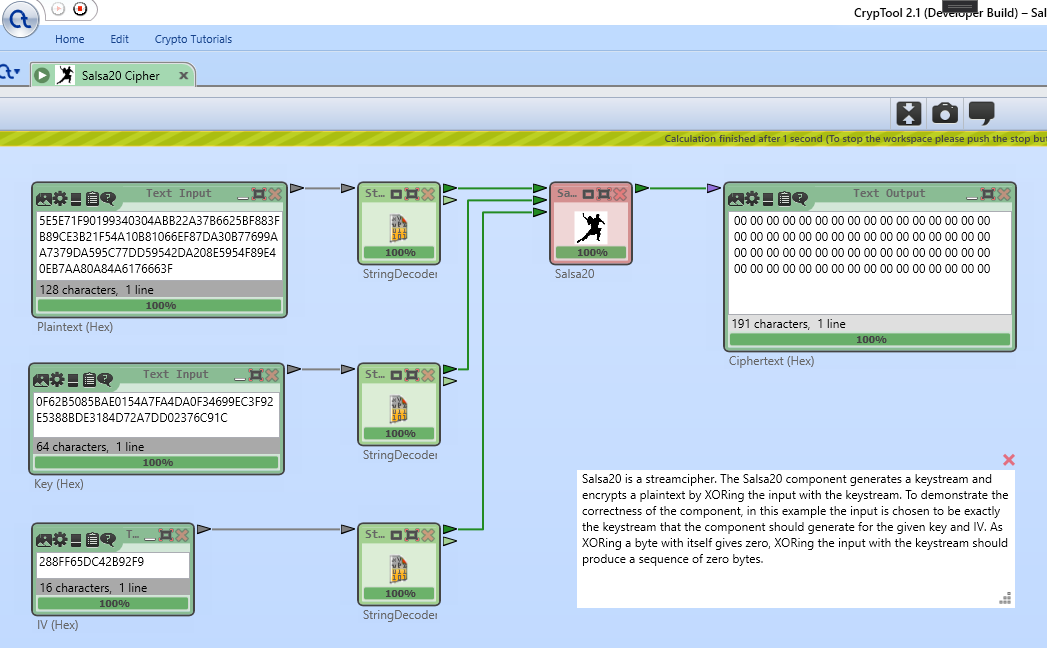
\includegraphics[width=\textwidth]{figures/ct2/salsa-crop.png}
\caption[Salsa20 CT2 template]{CT2 template for the already existing Salsa20 plugin}
\end{figure}

CrypTool 2 already has a plugin for the Salsa20 cipher but without a visualization.

During my work on the ChaCha visualization, I thought about how I could reuse my code for the ChaCha visualization to create a visualization for the Salsa20 cipher. I figured that it would not be as straight-forward as I assumed in the beginning since the visualization goes very into detail and thus the differences would involve at least different XAML code. For example, since the state is built up differently, the visualization about the state matrix initialization would need to be adapted. Also, the quarterround is slightly different which also needs to be reflected in the visualization. 

Nonetheless, I think that most of the codebase used for the ChaCha cipher could be reused to create a Salsa20 visualization, especially the navigation system and how the intermediate results are stored and retrieved for visualization. I will further discuss this in Chapter \ref{chap:futureWork}.


%%%%%%%%%%%%%%%%%%%%%%%%%%%%%%%%%%%%%%%%%%%%%%%%%%%%%%%%%%%%%%%%%%%%%%%%
\section{Other CrypTool 2 Cipher Visualizations}
\label{sec:otherCT2CipherVisualizations}

In this section, I will discuss ideas that I got from existing CrypTool 2 cipher visualizations which were also created by students during their bachelor thesis.

\subsection{AES Visualization}
\label{sec:aesVisualization}

\begin{figure}
\label{fig:aes}
\centering
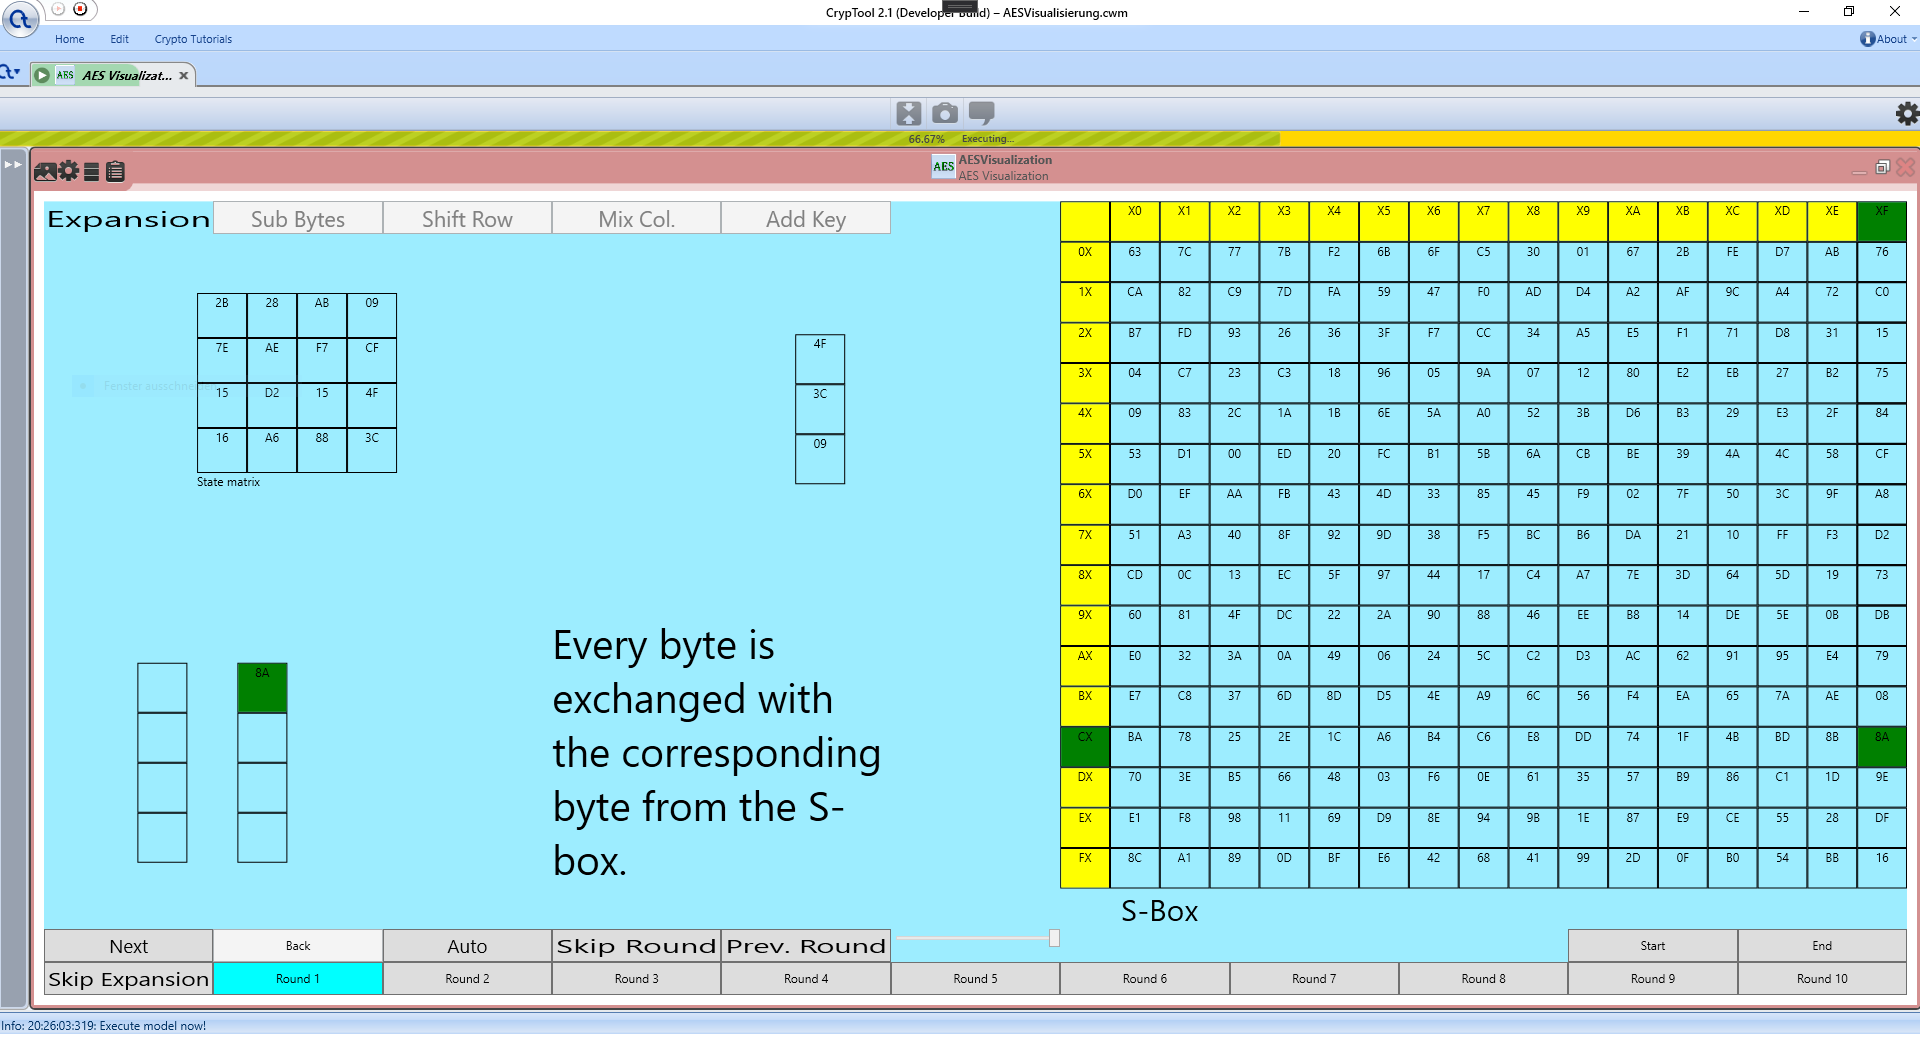
\includegraphics[width=\textwidth]{figures/ct2/aes.png}
\caption{AES visualization plugin}
\end{figure}

Matthias Becher created a visualization for the AES cipher during his bachelor thesis in 2016. It was the visualization of which I took the most inspiration for my own implementation. I also read through his bachelor thesis to see how he solved some of the problems that I encountered. For example, he wrote the following:

``The first big decision that had to be made was whether the states after each encryption operation would be calculated during the visualization or precalculated and stored at the start of the execution. One feature the plugin should have was to not only jump ahead to later operations but also to go back to previous ones. That means if the values were calculated during the visualization every time you went back they would have to be recalculated from the start. Therefore, I decided to precompute and store results of each operation in an array of byte arrays..'' \cite{aesthesis}

I came to the exact same conclusion that the values need to be precalculated for the reasons he mentioned.

Looking through his visualization, I liked how he changed the background of the elements to catch the user's attention. This is shown in Figure \ref{fig:aes}. I have used a similar mechanic during the ChaCha hash function visualization where I put a light blue background onto the state elements which will be used as the quarterround input. Also during the quarterround, I extensively used background coloring to tell the user where he should pay his attention.

Another thing I adopted from his visualization was the navigation in the top-left corner. I placed my page navigation there.

What I wanted to do differently in my navigation was to not show so many buttons all the time to the user. I was quite overwhelmed by all the buttons in the bottom navigation bar on the start even though they were disabled. Therefore, on pages which have no actions, I had no buttons in the bottom row. On pages with actions, a simple slider with a previous and next button did suffice. For the ChaCha hash function, which needed additional navigation, my navigation bar looked similar but still felt in my opinion less crowded, especially because I did not use buttons for every single round but a text input .

Further, I was confused why I could not use the ``Back'' button during the ``Expansion'' or ``Encryption'' step. For my plugin, I wanted to let the user navigate to any step in the visualization fairly simple. To achieve this, I needed to make sure that the user knows where he is and where he needs to click to go to a particular step. To give the user the information he needed, I used the dedicated page navigation in the top-left corner which stays the same on every page and tells the user on which page he currently is with bold font. Further, I numbered every single action on each page together with an action text input and how many actions a page has. The text input makes it possible for the user to immediately jump to an action.

\subsection{DES Visualization}
\label{sec:desVisualization}

\begin{figure}
\label{fig:des}
\centering
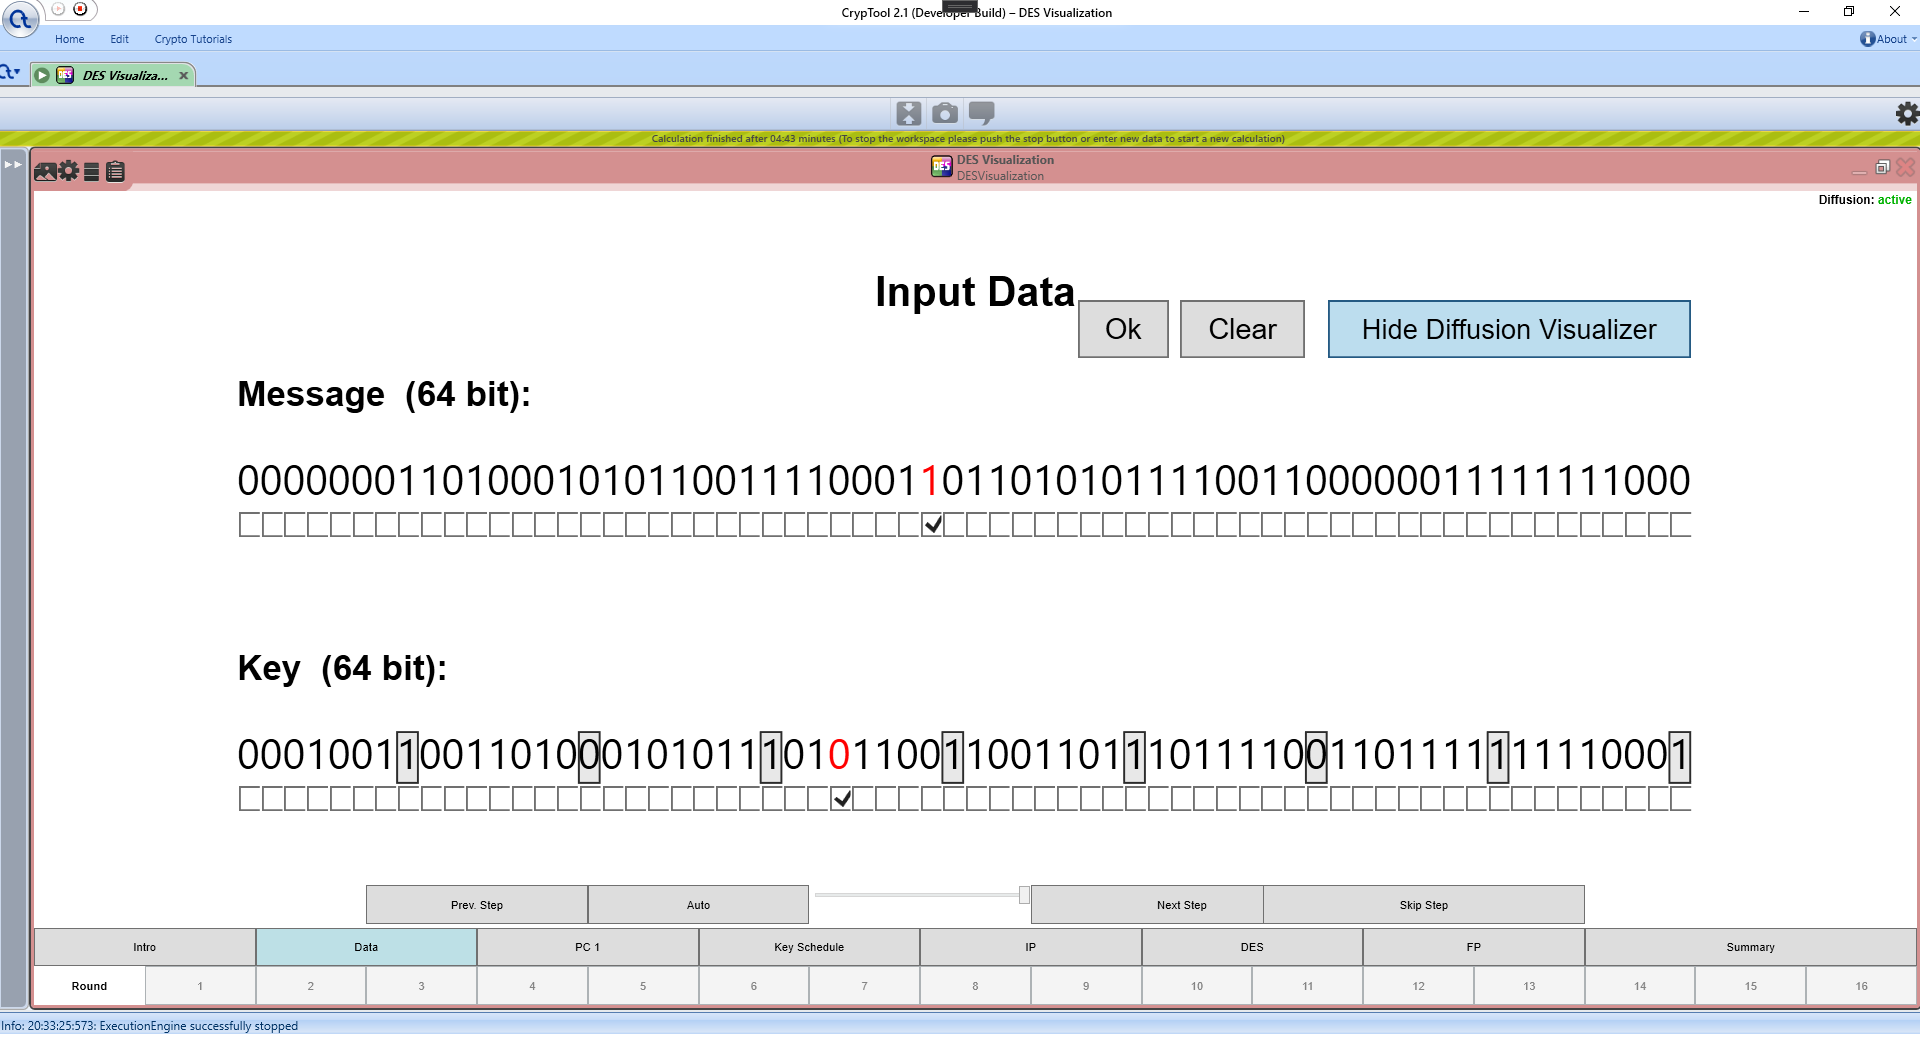
\includegraphics[width=\textwidth]{figures/ct2/des.png}
\caption{DES visualization plugin}
\end{figure}

The DES visualization was also created by a student, Lars Hoffman, for his bachelor thesis. His approach to visualizing the diffusion had the most influence on my diffusion visualization. In Figure \ref{fig:des}, you can see the page on which the user can flip bits to activate diffusion. The message and key with flipped bits will then be used to show the diffusion property of DES. 

Throughout the visualization, all values are shown in binary. This makes it possible to just mark flipped bits red since if a bit is marked red, we immediately know the value of the diffusion run (we just flip the red bit). 

I used the same coloring approach but noticed that since the ChaCha cipher was using longer keys and 512-bit blocks compared to the 64-bit blocks of DES, I needed to use hex strings for my values to save canvas space. This lead to a loss of information about the value of the diffusion run if only marking red the hexadecimal characters which are different. Therefore, I combined the usage of red color together with showing both values in two rows. In the row for the diffusion value, the difference is still marked red for easier visual recognition. This is shown in Figure \ref{fig:chachahash.mid.qr.with.diffusion}.

\subsection{Avalanche Visualization}
\label{sec:avalancheVisualization}



  %%%%%%%%%%%%%%%%%%%%%%%%%%%%%%%%%%%%%%%%%%%%%%%%%%%%%%%%%%%%%%%%%%%%%%%%
\chapter{Results}
\label{chap:Results}

\hyperref[sec:index]{Chapter}\index{chapter}~\cite{Hanser2019energy}. In \autoref{chap:Results}, \autoref{sec:section}, we will see bla, specifically in \autoref{sec:subsection} this will be emphasized. \Blindtext[2]
%%%%%%%%%%%%%%%%%%%%%%%%%%%%%%%%%%%%%%%%%%%%%%%%%%%%%%%%%%%%%%%%%%%%%%%%
\section{Section}
\label{sec:section}

\Blindtext[6]
%%%%%%%%%%%%%%%%%%%%%%%%%%%%%%%%%%%%%%%%%%%%%%%%%%%%%%%%%%%%%%%%%%%%%%%%
\subsection{Subsection}
\label{sec:subsection}

\Blindtext[3]
%%%%%%%%%%%%%%%%%%%%%%%%%%%%%%%%%%%%%%%%%%%%%%%%%%%%%%%%%%%%%%%%%%%%%%%%
  % !TeX spellcheck = en_GB

%%%%%%%%%%%%%%%%%%%%%%%%%%%%%%%%%%%%%%%%%%%%%%%%%%%%%%%%%%%%%%%%%%%%%%%%
\chapter{Conclusion}
\label{chap:conclusion}

This chapter finishes the thesis by summarizing its main points. It also includes suggestions how the plug-in could be further improved in the future.

\section{Summary}
\label{sec:summary}

This section gives a high level overview over the main points of this thesis. \\
In Section \ref{sec:implementationDetails}, the implementation is described. The section gave a detailed overview over how the plug-in was designed to meet the goals defined in Section \ref{sec:goals}. Section \ref{sec:encounteredProblems} described previous architectures and which problems they had.\\
The main point of this thesis is the description how the current implementation meets these goals and how the problems which occurred during development were solved.

\subsubsection{Goals}

Three goals which the plug-in should meet were defined.

\begin{enumerate}[label=(\labelenum{G}{{\arabic*}}), wide, labelwidth=!, labelindent=0pt]
\setlength{\parskip}{0pt}
    \item \textbf{Easy-to-understand visualization of the encryption process}\\
    The first goal was met by creating a simple but thought-through user interface for the plug-in visualization.
    
     The visualization is split into five pages in the following order:\\
      A landing page, an overview page, a page to adjust diffusion settings, a page which visualizes the state setup and a page which visualizes the ChaCha hash function.\\
     Splitting the visualization up into five different pieces made it easier to let the user focus on a single step of the encryption process. This also made it possible to have a new page layout for each step without confusing the user because each page is presented as an individual piece. A new page layout for each step was useful because we then were not restricted to a single layout for the whole visualization. Presenting the pages as individual pieces starts with the clear cut from the landing page to the overview page using the page navigation bar in the top-left of each page. Since at the landing page, only the page navigation bar at the top-left is shown, the user knows that he must use it to advance. After using it, it is clear to the user that this is the place where he can navigate between pages.
     
     Each page tells the user with descriptions what it is about. If a page has what we called actions, the user has access to a slider with buttons in the bottom with which he can navigate within a page. At the bottom-right, the total actions a page has (which corresponds to in how many different states a page can be) is shown together with a text input which shows the current action index.
     
     Using that text input makes it possible to skip to a certain action. Since the user will not know which action corresponds to which page state when using the plug-in for the first time, additional buttons are shown above the slider which bring the user immediately to important intermediate steps. Looking at the current action index, the user now knows what he has to type in there to immediately jump to that action again. This indirectly helps to better understand the cipher because it enables student and lecturers to talk about a specific step using the action index number.
     
     The state setup and the hash function were visualized with attention to detail. \\
     During the state setup, each parameter is encoded separately and each encoding step is described. During the hash function, the quarter-round circuit diagram makes it possible to show the intermediate results in an intuitive way by placing them above the circuit lines. Intermediate results were important to let the user comprehend every single step of the keystream block generation. Further, background coloring helps to show which elements are used to calculate the next value or which state entries are currently in use by the quarter-round function.
     
     \item \textbf{Visualization of the diffusion property}\\
     The diffusion property is visualized by letting the user enter alternative values on the Diffusion page. Since the ChaCha keystream is independent of the plaintext, the user can only use alternative values for the key, counter and IV.
     
     It was important to easily be able to flip bits. Thus, the user can not only enter the explicit alternative value but also the XOR.
     
     An example on the same page informs the user what he can expect for the next pages if he activates diffusion by flipping at least one bit. It shows that he can chose between two views: \\
     A view where he can see both values and a view which can be activated with the button in the top-right corner to only show the XOR between both values.\\
     The values are always shown in hexadecimal and a character which has changed is marked red for easier visual recognition. These two different views were important because when studying the diffusion property of a cipher, one is more interested in the difference between two keystreams instead of their actual values. On the other hand, having access to the concrete values could also be useful thus both views were implemented instead of just one.
     
     Additionally, the percentage of flipped bits is shown below the state at the end of each quarter-round in the ChaCha hash function page.
     
     \item \textbf{Support for all variants of the cipher family}\\
     The support to choose the amount of rounds and the version (original version by Bernstein or IETF version) was implemented by adding appropriate settings to the plug-in. The inputs are then validated accordingly. This means that if the user has chosen the original version by Bernstein, he must enter a 64-bit counter and a 64-bit IV. If he has chosen the IETF version, he must enter a 32-bit counter and a 96-bit IV. The plug-in will not start with wrong inputs. Instead, it will show an error message with the expected size for the input and its actual size.
     
     The visualization works not much different with a 128-bit or 256-bit key. It is mentioned that if using a 128-bit key is used, it will be concatenated with itself. This is done in the step where the encoded key is put into the state.\\
     To reflect the chosen version, only the state setup is slightly different. The last row of the state is partitioned differently.
  \end{enumerate}

\subsubsection{Main problems (P) and their solutions (S)}

Two main problems were encountered while developing the plug-in.

\begin{enumerate}[label=(\labelenum{P}{{\arabic*}}), wide, labelwidth=!, labelindent=0pt]
\setlength{\parskip}{0pt}

\item \textbf{Architecture}\\
The first problem was to find out how the architecture behind the user interface should be laid out to not hinder further development. This means that it was not straight-forward to know how all systems (user interface, the cipher implementation, navigation, storage and retrieval of intermediate values) should interact without introducing hard-to-debug bugs in the long run.

\item \textbf{Performance}\\
The second problem was the overall performance of the plug-in. It was caused by the desire to let the user navigate to any step within a page. Letting the user navigate from any step to any step meant that the navigation system must support a lot of possible transitions in a reasonable time.

\end{enumerate}

\begin{enumerate}[label=(\labelenum{S}{{\arabic*}}), wide, labelwidth=!, labelindent=0pt]
\setlength{\parskip}{0pt}

\item \textbf{MVVM design pattern}\\
The first problem was solved by following a design pattern. The MVVM design pattern was chosen because it was the most popular across the WPF community. 

Using a design pattern helped in solving a lot of problems in a very obvious way. Features which previously were implemented with a lot of code smells could now be implemented properly without increasing technical debt. \\
For example, before using a design pattern, the navigation system was spread across the whole code base. With the MVVM design pattern, the whole navigation system could be written as a single interface. A abstract view model class then implemented this interface. All other view models which had actions then just extended this base class without having to duplicate any navigational logic.

As mentioned in Section \ref{sec:Architecture}, extensive usage of data binding helped in decoupling the view code from the underlying architecture. Therefore, if some things in the view should change, almost no code in the architecture has to change if the MVVM design pattern is properly implemented. Previously, the view code was very rigid. Changing it took a lot of effort because it kept breaking the architecture behind it.

\item \textbf{Centralized navigation system}\\
The second problem was solved by reflecting on the performance problems previous navigation system implementations had and their underlying issues.

The problem of the first navigation system was that it was designed to execute the transitions in a linear manner (hence the name \textit{linear navigation system}). This meant that skipping a lot of actions would take a lot more time than skipping only a few actions because a lot more transitions needed to be executed for the larger skip. This resulted in taking more than 40 seconds to skip about 3000 actions on the ChaCha hash function page.

This was tried to solve by introducing caches. Even though the cache implementation brought the response time down to 200ms, it did not solve the problem to a satisfactory degree. It introduced inconsistencies regarding the performance because with it, it was not obvious to the user why some skips took longer than others. Before, one could easily see that larger skips took longer than smaller.

As described in Section \ref{sec:Architecture}, as a result, the navigation system was optimized to have a consistently good performance for any skip. This means that the overhead of the navigation system design should be approximately equal for any skip. This was possible with the centralized navigation system. Any transition would start with first going back to the first action and then from there straight to the destination action. Therefore, the start action does not matter because moving to the first action from any action is done in $O(1)$ and moving from the first action to any action is done in $O(1)$. This improved performance dramatically. The average response time was now 5 ms with a maximum response time of about 10 ms.


\end{enumerate}

\section{Future Work}
\label{sec:futureWork}

This section lists suggestions how the plug-in could be further improved to make it more useful for the audience of CrypTool 2.

\begin{enumerate}[wide, labelwidth=!, labelindent=0pt]
\setlength{\parskip}{0pt}

\item \textbf{Better overview over flipped bits at the end of each round}\\
At the end of the Avalanche visualization, the author provided an overview over the percentage of flipped bits at the end of each round. This overview is very useful because it shows how the amount of flipped bits goes up very fast to around 50\% and then stays near it which is exactly what one would expect from a good cipher.

Using a plot instead of the simple text which is updated at the end of each round was considered but due to canvas and time constraints, this idea was not further pursued. 

Nonetheless, integrating such an overview into the Diffusion page should be possible. This would need cipher execution while still on the page instead on page exit but this would not be a big problem since a button to start cipher execution would suffice. Therefore, this plot could be an addition instead of replacing the text below the state in the ChaCha hash function visualization.

\item \textbf{Improve performance during diffusion}\\
All measurements in Section \ref{sec:Architecture} were done with inactive diffusion since the performance during active diffusion improved in a similar manner. This means that thanks to the centralized navigation system architecture, moving to any action is still done in constant time even if diffusion is active.

The problem is that it takes around one or two seconds for each move (instead of around 5 ms if diffusion was inactive) which is quite annoying. We suspect that this is the case because the red color is implemented by creating an inline element for every character and marking it red if it is different.

An idea is to create a single element for every possible combination of color (black and red) and hexadecimal character ([0-9A-F]). Therefore, we would not need to create a new inline element for each character but could reuse the same in multiple places. If the performance issue results from the memory allocation, this approach should solve it. 

However, first attempts resulted in weird bugs. So fixing this will probably be the most difficult point in this list and could result in once again having to rethink some major design decisions.

\item \textbf{Automatic navigation}\\
The AES visualization includes a button labeled with ``Auto''. It lets the visualization run without further user interaction needed. A slider was provided to adjust the speed (see Figure \ref{fig:aes}). 

Such a button could be useful for the ChaCha visualization, too, especially for the page about the ChaCha hash function with its many actions.\\
Since asynchronous navigation is already in use for the action slider, implementing this feature could easily be integrated within the existing navigation system. Only page switches could maybe need some clever solutions since the action navigation is handled within each page thus navigating out of a page may not be straight-forward. 

In the AES visualization though, the automatic navigation does stop between each step (which roughly corresponds to a page in our visualization) so switching the page automatically may even not be desired.

\item \textbf{Salsa20 visualization}\\
As mentioned in Section \ref{sec:salsaCT2Plugin}, using the now existing codebase for ChaCha visualization to create a Salsa20 visualization would definitely increase the value gained from this thesis.

This would at least need adaption of the XAML code for the state matrix initialization and the quarter-round since ChaCha and Salsa20 differ in these aspects from each other. It would most likely even increase the value of the ChaCha visualization since both ciphers could then be compared side-by-side. Comparing them and their diffusion property should be very easy due to the very similar visualization.

\item \textbf{Localization and online help}\\
Currently, most texts are only localized in English. Only the memo fields, component labels and plaintext value are also available in German.\\
This will be changed in the near future. Then also an online help entry for the ChaCha plug-in will be available. The online help appears when pressing F1.

\end{enumerate}

%%%%%%%%%%%%%%%%%%%%%%%%%%%%%%%%%%%%%%%%%%%%%%%%%%%%%%%%%%%%%%%%%%%%%%%%  

% This ensures that the subsequent sections are being included as root
% items in the bookmark structure of your PDF reader.
\bookmarksetup{startatroot} 
\backmatter

  % \begingroup 
  %   \let\clearpage\relax 
  %   \glsaddall
  %   \printglossary
  % \endgroup

  \printindex
  \label{sec:index}
  
  \printbibliography
  
\end{document}